
\chapter[A Proposta]{A PROPOSTA}

A proposta deste trabalho é criar uma ferramenta capaz de produzir projetos de gamificação, a ferramenta servirá para automatizar o processo de criação dos projetos, simplificar e incentivar a inserção de gamificação no cotidiano das pessoas que tem interesse pelo tema e querem aplicá-lo as suas vidas. Este capítulo está estruturado da seguinte maneira: introdução, onde será feita uma contextualização sobre o porque de se construir uma ferramenta com tal propósito e construção da ferramenta, onde será descrito o processo de construção da ferramenta.           

\section{Introdução}

 

Segundo Yu-Kai Chou \cite{chou2015actionable} gamificação é o ato de cuidadosamente aplicar ao mundo real e as atividades produtivas e os elementos divertidos e envolventes dos jogos, o que torna o ato de gamificar mais complexo que apenas incorporar elementos de jogos em outros contextos, gamificar é mais sobre  motivar pessoas e menos sobre pontos e troféus \cite{chou2015actionable}, isso faz com que gamificação seja um tema que diz respeito ao ser humano, gamificação é um novo olhar sobre motivação e como motivar pessoas e mudar vidas, vai além de inserir elementos de jogos em contextos fora de jogos, gamificar é trazer pra vida real o incentivo natural que se tem ao jogar jogar um jogo, é tentar despertar em atividades do cotidiano a mesma sensação que se tem ao jogar.

Ninguém tem que jogar um jogo, as pessoas tem que trabalhar e pagar sua contas, elas não são obrigadas a jogar, mas jogam \cite{chou2015actionable} e se sentem motivadas, felizes e incentivadas a dar o melhor de si quando estão jogando. Porque as pessoas se sentem motivadas a jogar mas não sentem a mesma motivação na vida real, para conquistar objetivos? O que falta? Motivação? Disciplina? Um modelo de incentivo que funcione? O jogo gera mais esperança de sucesso nas pessoas, em comparação ao jogos, a realidade não demonstra esperança \cite{mcgonigal2011reality}, por isso as pessoas têm tanto interesse em jogar e não dispõem do mesmo interesse para realizar ou concluir tarefas cotidianas ou conquistar uma meta a longo prazo, mas é possível deixar esses aspectos da vida mais divertidos e motivadores, jogos podem mesmo mudar vidas e motivas pessoas, então a gamificação também pode. Porque não construir uma ferramenta que dê suporte a tantas oportunidades de aplicar a vida real a motivação instrisicamente ligada aos jogos? Uma ferramenta capaz de dispensar do usuário todo o conhecimento prévio que ele precisaria ter para construir um projeto de gamficação que tivesse chances de dar certo? Uma ferramenta que motive as pessoas a mudar algo que pode ser modificado fazendo uso de gamificação, pode ser a forma de lecionar uma aula, um percurso utilizado em um tratamento de reabilitação motora, pode ser o hábito da falta de estudo diário, muita coisa pode ser fruto de um projeto de gamificação.

Há algumas décadas têm-se estudado a motivação intrinsecamente ligada ao jogo e como aplicá-la em outras áreas com o mesmo sucesso\cite{chou2015actionable}. Mas motivar apenas não basta, motivação acaba, é preciso pensar maneiras de manter a motivação, criar um ciclo onde além de motivadas as pessoas permaneçam disciplinadas, mas não por obrigação, e sim porque sentem vontade de sempre seguir adiante. Por isso a proposta de criar uma ferramenta que motive o usuário do início ao fim e o auxilie a  conquistar uma meta de maneira disciplinada e divertida e que não pareça uma obrigação, uma ferramenta que consiga agregar os pontos positivos da gamificação e aplicá-los a vida real. A ferramenta existirá para que o nivel de conhecimento exigido atualmente para se criar um projeto de gamificação seja diminuído. A pessoa não vai precisar estudar gamificação para conseguir montar um projeto de gamificação, ela fará isso de maneira guiada e intuitiva, prentende-se também que com o uso do sistema, o usuário com algum grau de conhecimento do assunto tenha sua produtividade elevada no momento da construção do projeto de gamificação. Para que o sistema resulte em bons projetos ele será constítuido de elementos que darão suporte a uma gamificação coerente.





\newpage

\section{Construção da ferramenta}

A figura X representa os componentes internos que serão utilizados para dar forma a ferramenta, cada cubo da figura representa os cores drives, técnicas de gamificação e os atributos das técnicas de gamificação. Os cores drives, representados como a parte superior do cubo, são as unidades principais do framework e serão também o principal componente da ferramenta, as técnicas de gamificação, representadas como o lado esquerdo do cubo, compõem as unidades principais, os atributos, representados como o lado direito do cubo, compõem as técnicas de gamificação. Como a ferramenta tem como propósito da construção de projetos gamificação que motivem os seus usuários ela terá o usuário como foco principal, como indicado na figura, o design focado no ser humano \cite{chou2015actionable} ou design centrado no usuário \cite{JanakiMythilyKumar and Mario Herger}, indica que o processo de concepção e desenvolvimento da gamificação será focado no usuário e nas suas motivações. 

\begin{figure}[h]
	\centering
	\label{fig01}
		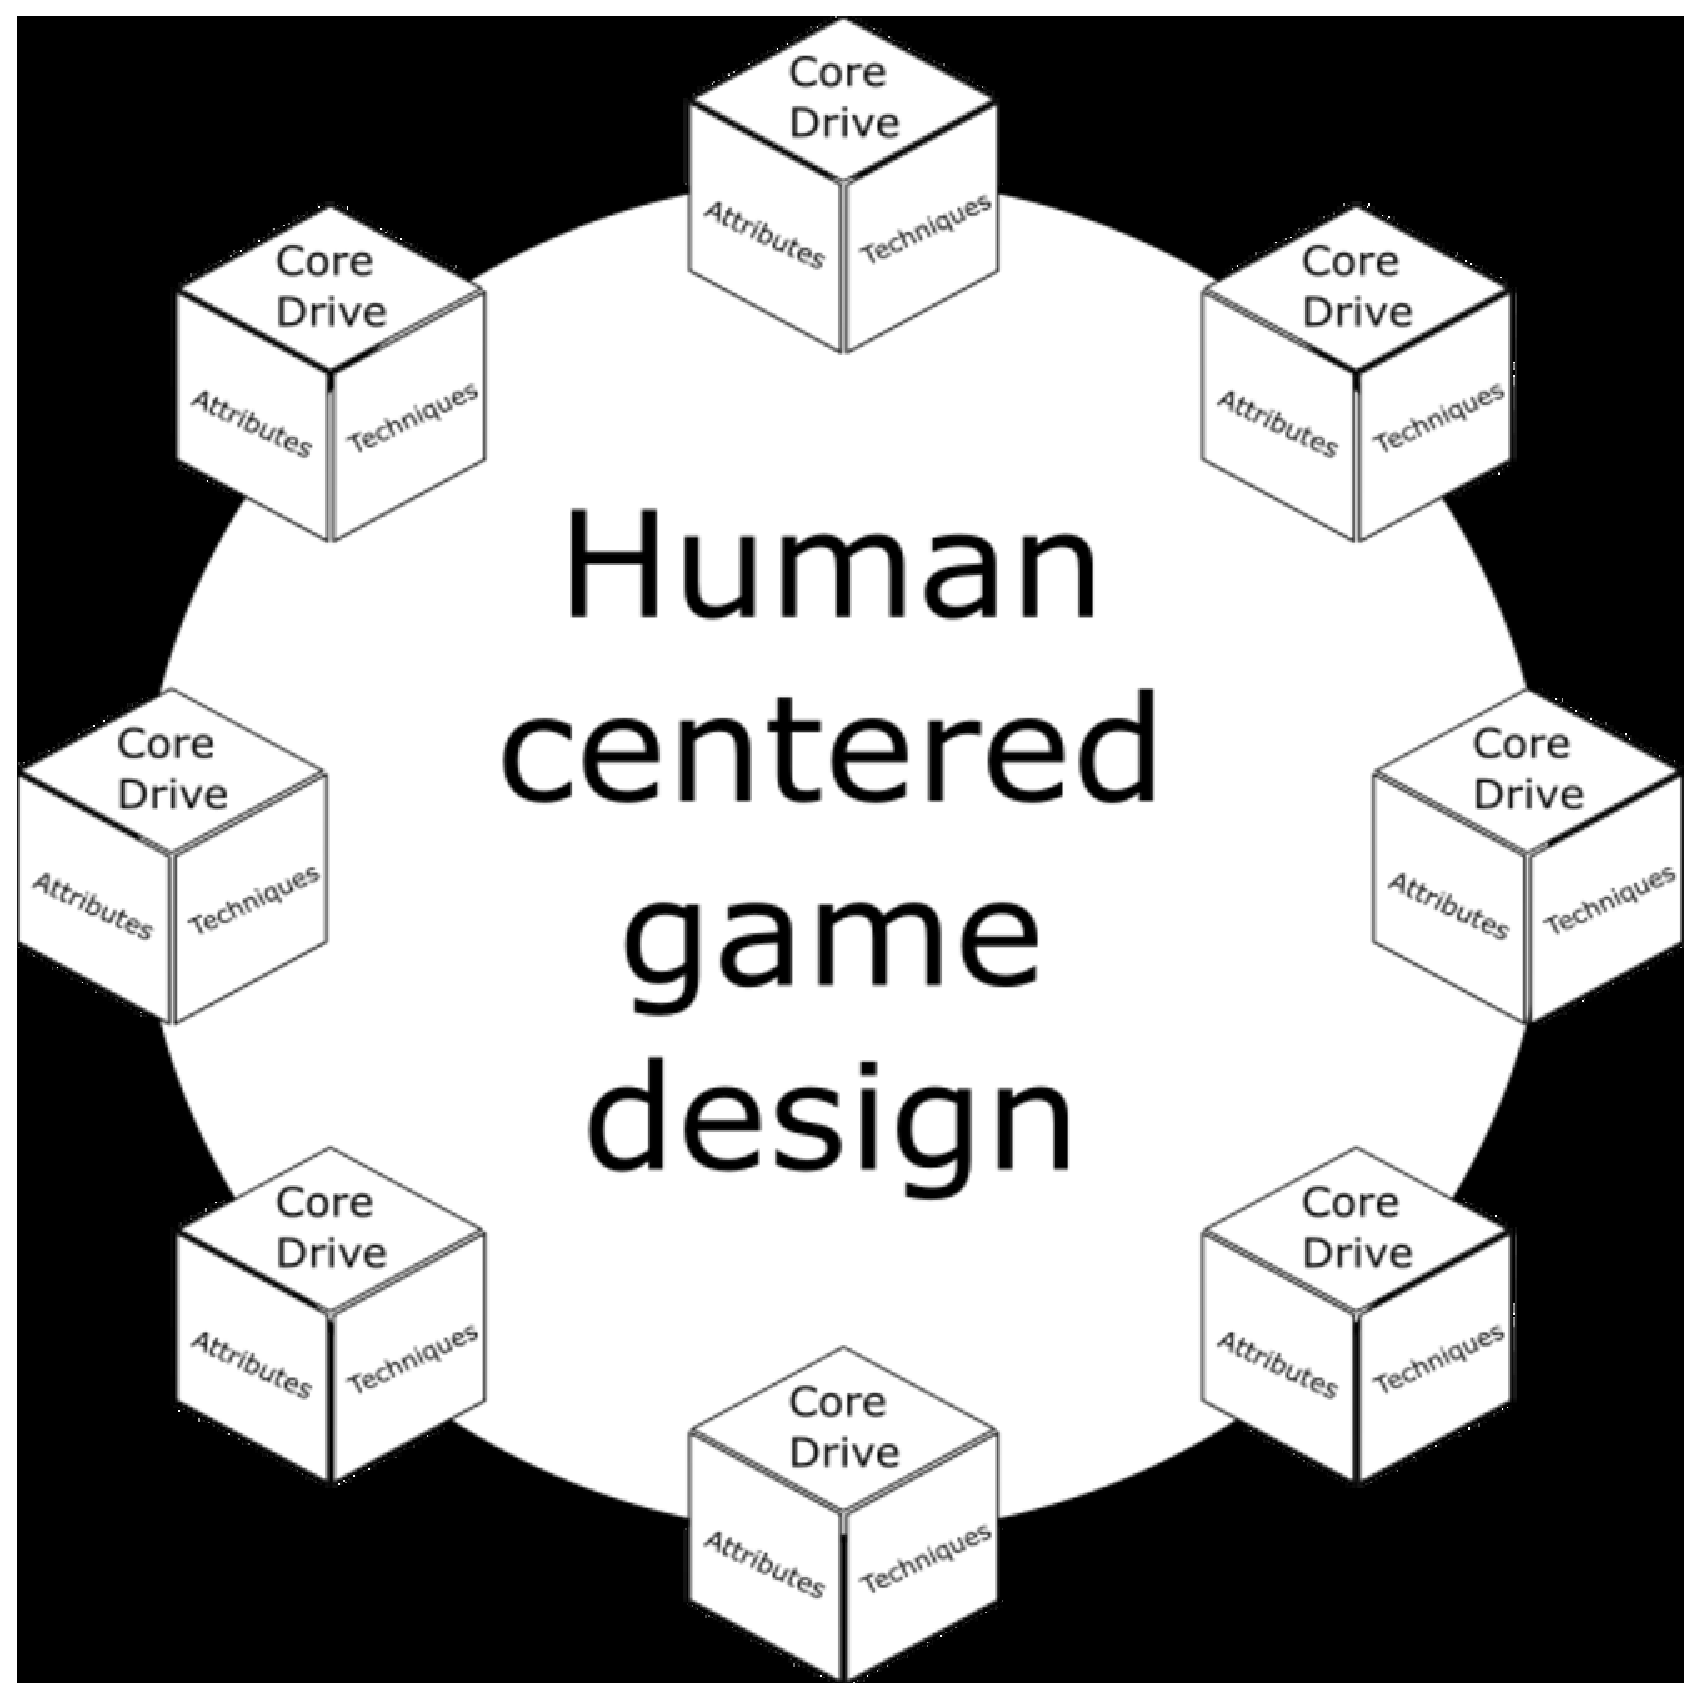
\includegraphics[keepaspectratio=true,scale=0.5]{figuras/hcgd.eps}
	\caption{Composição da Ferramenta}
\end{figure}


Para que a ferramenta possa ser construída de maneira adequada e que proporcione ao usuário uma experiência bem sucedida na criação do seu projeto de gamificação, o framework octalysis foi escolhido como alicerce para a construção da mesma, as unidades principais do framework juntamente com as técnicas de gamificação existentes estão bem alinhadas com o principal próposito da ferramenta. Yukai-Chou utiliza as unidades principais do framework para motivar os usuários, e as técnicas de gamificação para representar elementos de jogos, mas as técnicas possuem mais de uma função, elas são utilizadas também para intensificar a motivação representada pela unidade principal da qual fazem parte. O emprego correto das mesmas na construção do projeto de gamificação produz um resultado mais satisfatório, como gamificação é o ato de aplicar elementos de jogos em contexto fora de jogo, as técnicas de gamificação representam a ligação entre o contexto de não jogo ao contexto de jogo. Para que uma gamificação produza um bom resultado as técnicas de gamificação devem ser utilizadas de maneira a se complementarem.


As oito unidades principais do octalysis possuem uma descrição e são compostas por inúmeras técnicas de gamificação, já as técnicas de gamificação possuem uma descrição, mas não é especficado qual a sua composição, para construir a ferramenta definiu-se então um conjunto de atributos irão compor as técnicas e foi realizado um mapeamento que indicará se há relacionamento entre as técnicas e como isso influencia na construção do projeto de gamificação. Atualmente não há uma definição formal de um conjunto mínimo de atributos que devem estar presentes para que uma técnica seja implementada corretamente e não havia um mapeamento que informasse ao construtor do projeto de gamificação como as técnicas se relacionam, se é possível implementar todas de uma vez, se a implementação de uma afeta a implementação de outra, não há uma definição de como deve ser o relacionamento entre as técnicas de gamificação e isso acarreta uma dificuldade para identificar se o projeto de gamificação está sendo construído corretamente, não há também como identificar se uma técnica de gamificação está ligada a mais de uma unidade principal, para obter essa relação das técnicas entre si e das técnicas entre as unidades principais foi realizado o mapeamento das técnicas de gamificação, inicialmente levantou-se as unidades principais e as técnicas de gamificação pertencentes, porém, a primeira fonte de informação não continha todas as técnicas de gamificação presente no octalysis, então a busca foi extendida a outros meios, já que a informação sobre o framework não se encontra centrada em um só lugar. Cada técnica é composta por um identificador representado por uma, seguido de um número, 10 narrativa, por exemplo, e uma descrição, para facilitar o entendimento da técnica, atualmente além das oito unidades principais foram mapeadas 43 técnicas de gamificação.

As técnicas de gamificação tem uma descrição simples e intuitiva, é fácil entender o que a técnica faz e o que ela pretende motivar no usuário, mas é um conhecimento muito ligado a experiência pessoal de quem propôs a existencia e o uso da técnica, quando se faz necessário realizar a implementação, tirar do campo das idéias e colocar em prática, esse conhecimento teórico não é suficiente, porque está muito ligado ao conhecimento adquirido ao longo dos anos pelo especialista em gamificação, e a proposta aqui é justamente tornar a gamificação acessível também a não especialistas. Para tornar a implementação das técnicas mais tangível, foi definifo um conjunto de atributos caracterizadores, que tornam as técnicas de gamificação passíveis de implementação sem que elas percam a identidade ou o foco principial pertecentes a elas. O conjunto de atributos definidos para compor a estrutura interna das técnicas são alguns dos indicadores de engajamento definidos por \cite{fredericks2004}, Fredericks divide os engajamentos em três tipos, o engajamento emocional, que trata, por exemplo, de emoções como alegria, interesse e raiva, o engajamento comportamental, que trata de indicadores de conduta, tais como, esforço, atenção e persistência e o engajamento congnitivo, que trata, por exemplo, de flexibilidade para resolver um problema, concentração e domínio. Engajamento também pode ser interpretado neste contexto como envolvimento, cada tipo de engajamento possui alguns indicadores, os indicadores caracterizam os tipos de engajamento e foram escolhidos aqui também para caracterizar as técnicas de gamificação, tal como se fossem adjetivos caracterizando as técnicas de gamificação.  A estrutura interna das técnicas é igual, independente da técnica de gamificação em questão. Os indicadores escolhidos para compor a estrutura interna das técnicas são: 

\begin{itemize}
\item  \textbf {Envolvimento com o trabalho:}  Mensura a quantidade de envolvimento com a gamificação que a técnica exigirá do usuário.
\item  \textbf {Participação:}  Mensura quanta participação efetiva na gamificação a técnica exigirá do usuário
\item  \textbf {Atenção:}  Mensura quanta atenção a gamificação exigirá do usuário.
\item  \textbf {Persistência:} Mensura quão persistente o usuário será para obter resultados no projeto de gamificação. 
\item  \textbf {Domínio:} Mensura a quantidade de maestria que o usuário precisará dispor para executar a técnica de gamificação. 
\item  \textbf{Social:} Mensura a quantidade de envolvimento social que a técnica dispõe para o usuário e quão social a técnica pode ser.
\end{itemize}


Cada indicador representará um atributo da técnica de gamificação e receberá uma valor que representa o grau de pertinência à técnica de gamificação, os valores variam de um a cinco e serão concedidos de acordo com a escala de Likert. A escala de Likert  \cite{arruda200} utilizada possui cinco itens: 

\begin{itemize}
\item  \textbf {1 - Muito aquém:} O atributo influência fracamente a técnica de gamificação
\item  \textbf {2 - Aquém:} O atributo influencia aquém do normal a técnica de gamificação
\item  \textbf {3 - Suficiente / Normal:} O atributo influencia de forma suficiente (normal) a técnica de gamificação
\item  \textbf {4 - Além:} O atributo influência além da normal a técnica de gamificação
\item  \textbf {5 - Muito além:} O atributo influencia plenamente a técnica de gamificação
\end{itemize}


\begin{figure}[h]
	\centering
	\label{fig01}
		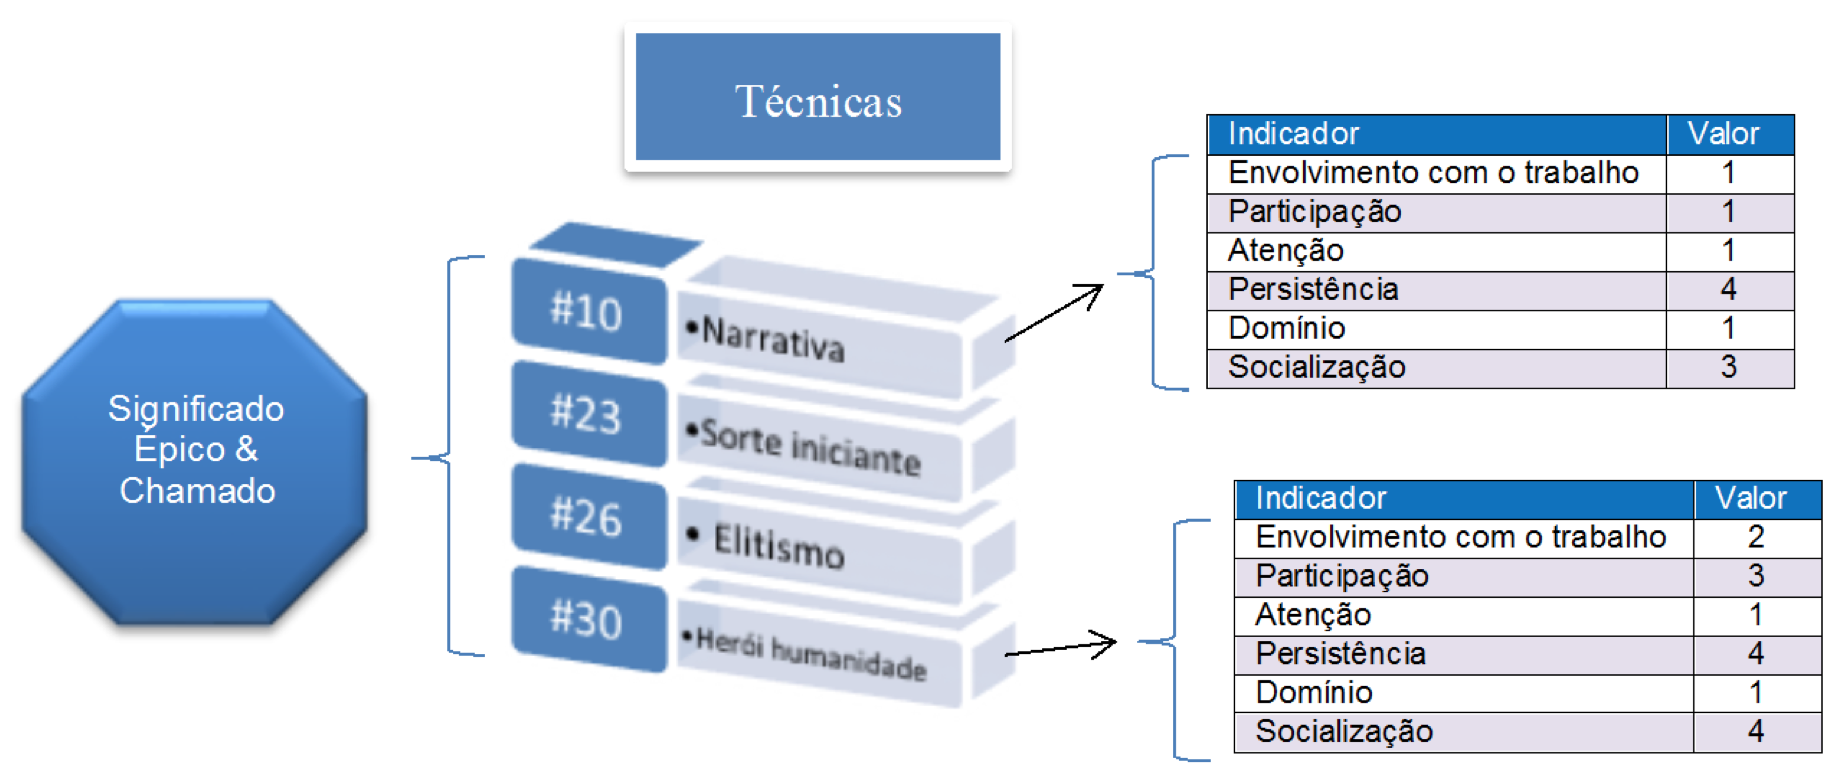
\includegraphics[keepaspectratio=true,scale=0.5]{figuras/mapeamento.eps}
	\caption{Estrutura interna da técnica de gamificação}
\end{figure}

Os atributos têm duas funções, caracterizar as técnicas de gamificação e espelhar o envolvimento do usuário com a gamificação, por exemplo, se a técnica exige do usuário muita atenção e persistência a gamificação também exigirá. Com a definição dos atributos formadores das técnicas é possível visualizar a estrutura interna da ferramenta em si. A ferramenta será composta da unidades principais do octalysis, das técnicas de gamificação e dos atributos das técnicas, os indicadores de engajamento. 

Após ser feito o mapeamento de todas as técnicas de gamificação existentes no framework é necessário mapear a ligação entre as mesmas, como mapeamento das técnicas já foi realizado e todos os indicadores receberam os valores pertinentes, o próximo passo é identificar se existe ligação entre as técnicas e se a implementação de uma pode exercer influência positiva ou negativa sobre outra, influenciando a construção do projeto de gamificação que o usuário esteja realizando.



